\chapter{Arquitectura da consola}
\label{chap:arquitectura}

\lettrine{N}{este} capítulo describiremos os diferentes compoñentes hardware da consola,
a súa interacción e o mapa de memoria que emprega.
Ademais explicarase o rol doutros compoñentes fundamentais para o seu funcionamento que son implementados
non polo hardware da consola, senón polos seus cartuchos.
A comprensión destes compoñentes é necesaria para entender o funcionamento da consola para unha posterior
implementación en forma de software de emulación.

\section{Visión xeral da arquitectura}
\label{sec:vision-xeral}

A maior parte das funcionalidades da consola son implementadas nun só \acrshort{soc}.
A pesar de ser nomeado como \acrshort{cpu}, por exemplo no seu encapsulado,
este chip ademais da propia \acrshort{cpu} inclúe varias memorias e diferentes periféricos, ocupando
a \acrshort{cpu} soamente unha pequena porción do silicio.

\begin{figure}[hp!]
  \centering
  \begin{subfigure}[c]{0.35\textwidth}
    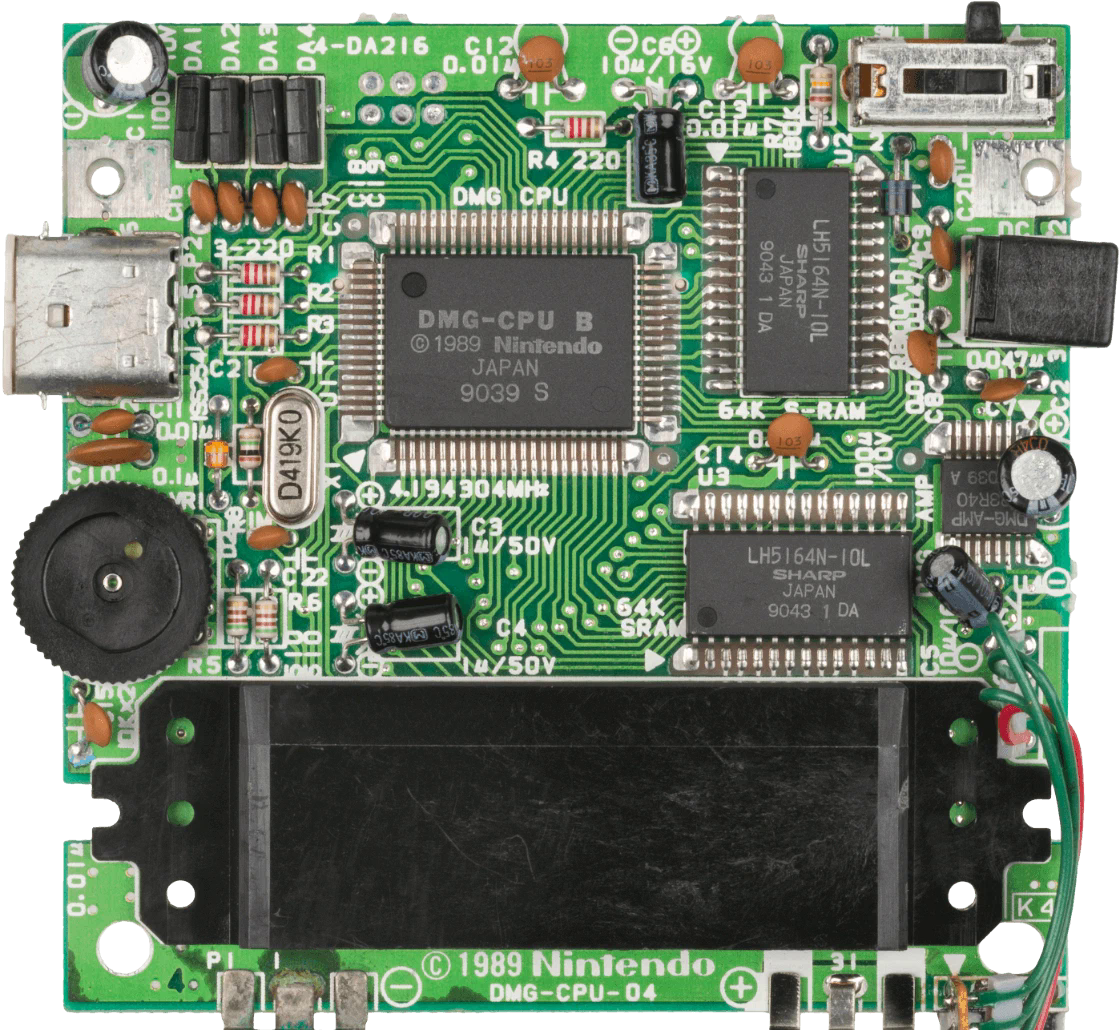
\includegraphics[width=\textwidth]{imaxes/motherboard_original.png}
    \caption{Placa base orixinal}
    \label{fig:motherboard-original}
  \end{subfigure}
  \hspace{0.02\textwidth}
  \begin{subfigure}[c]{0.35\textwidth}
    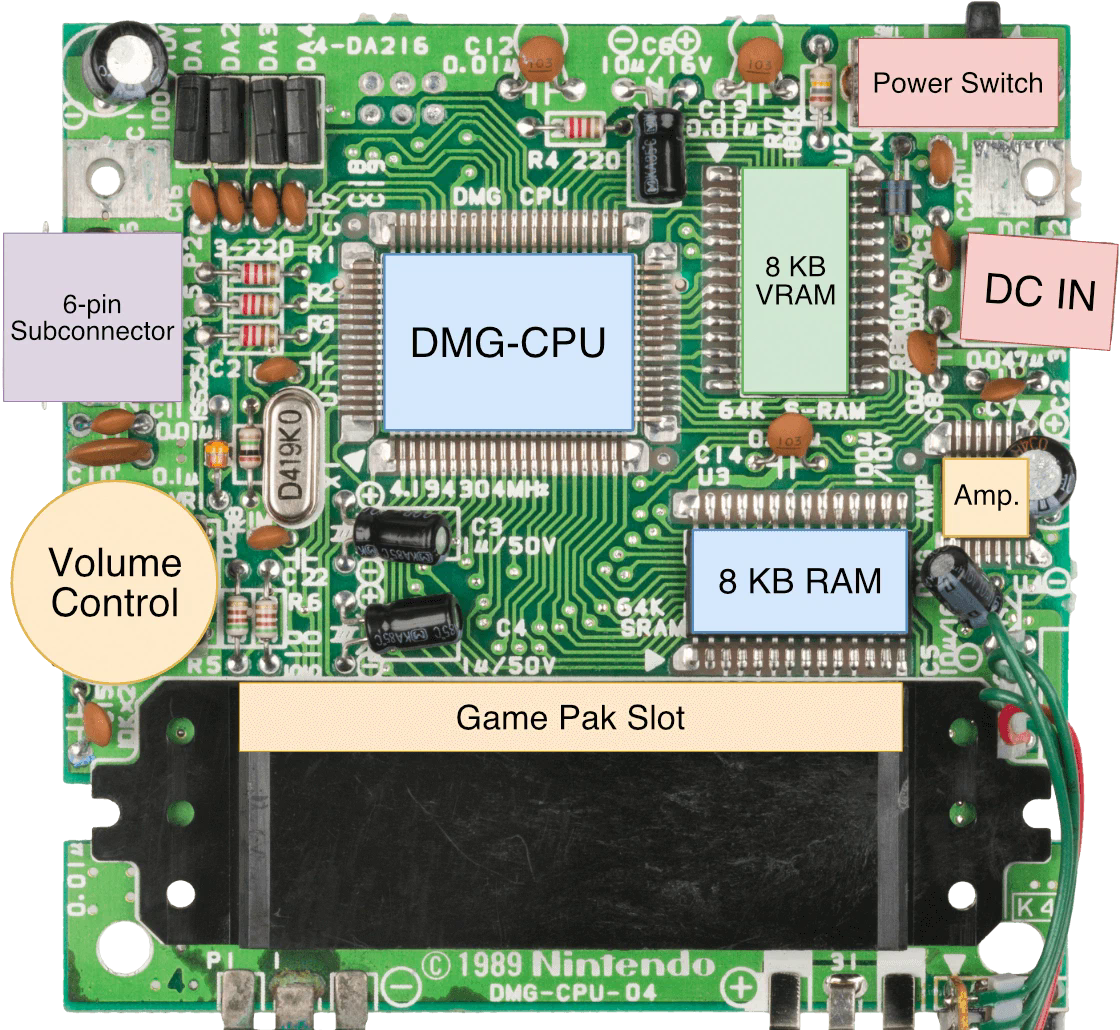
\includegraphics[width=\textwidth]{imaxes/motherboard_marked.png}
    \caption{Compoñentes principais sinalados}
    \label{fig:motherboard-marked}
  \end{subfigure}
  \caption{Placa base da Game Boy (\acrshort{dmg}), na que se aprecian o \acrshort{soc} (DMG CPU), a \acrshort{ram} e a \acrshort{vram} \cite{GekkioDatabaseDMGMainboard}}
  \label{fig:gameboy-motherboard}
\end{figure}

Dentro do \acrshort{soc} conviven a \acrshort{cpu}, a unidade de procesamento de píxeles (\acrshort{ppu}), a unidade de
procesamento de audio (\acrshort{apu}), os temporizadores, o controlador do joypad e o controlador de interrupcións.
Ademais conta con varias memorias, como a Boot \acrshort{rom}, a \acrfull{hram} e a \acrfull{oam}.

A Boot \acrshort{rom} é o primeiro programa que se executa ao acender a consola.
O seu cometido é preparar o sistema para a execución do programa principal provido polo cartucho.
Para iso inicializa varias zonas de memoria e rexistros dos periféricos.
Visualmente, amosa por pantalla unha sinxela animación co logotipo de Nintendo desprazándose ata 
o medio da pantalla e reproduce un son característico. Esta animación cumpre tamén unha
función de protección antipiratería.
Os xogos comerciais e validados por Nintendo requirían incluír na cabeceira da súa \acrshort{rom} unha copia
do logo de Nintendo. Durante a execución da Boot \acrshort{rom} realízase unha comparación entre os recursos
atopados aquí e os do cartucho. Se a comparación falla, a consola queda bloqueada e sen executar o xogo.
Este mecanismo foi usado por Nintendo para controlar que xogos se podían executar na súa consola.
Os distribuidores de cartuchos non autorizados afrontaban unha dobre penalización, xa que ao ter que incluír
o logo de Nintendo incorrían en dúas infraccións: a de marca rexistrada e a dos dereitos de autor.

Fóra do \acrshort{soc} sitúanse a memoria de traballo (\acrshort{wram}), a memoria de vídeo (\acrshort{vram}) e
a propia \acrshort{rom} do cartucho, que pode incluír ademais hardware específico (véxase
sección~\ref{sec:mbc}). A figura~\ref{fig:diagrama-arch} amosa a relación entre estes
compoñentes.

\begin{figure}[hp!]
  \centering
  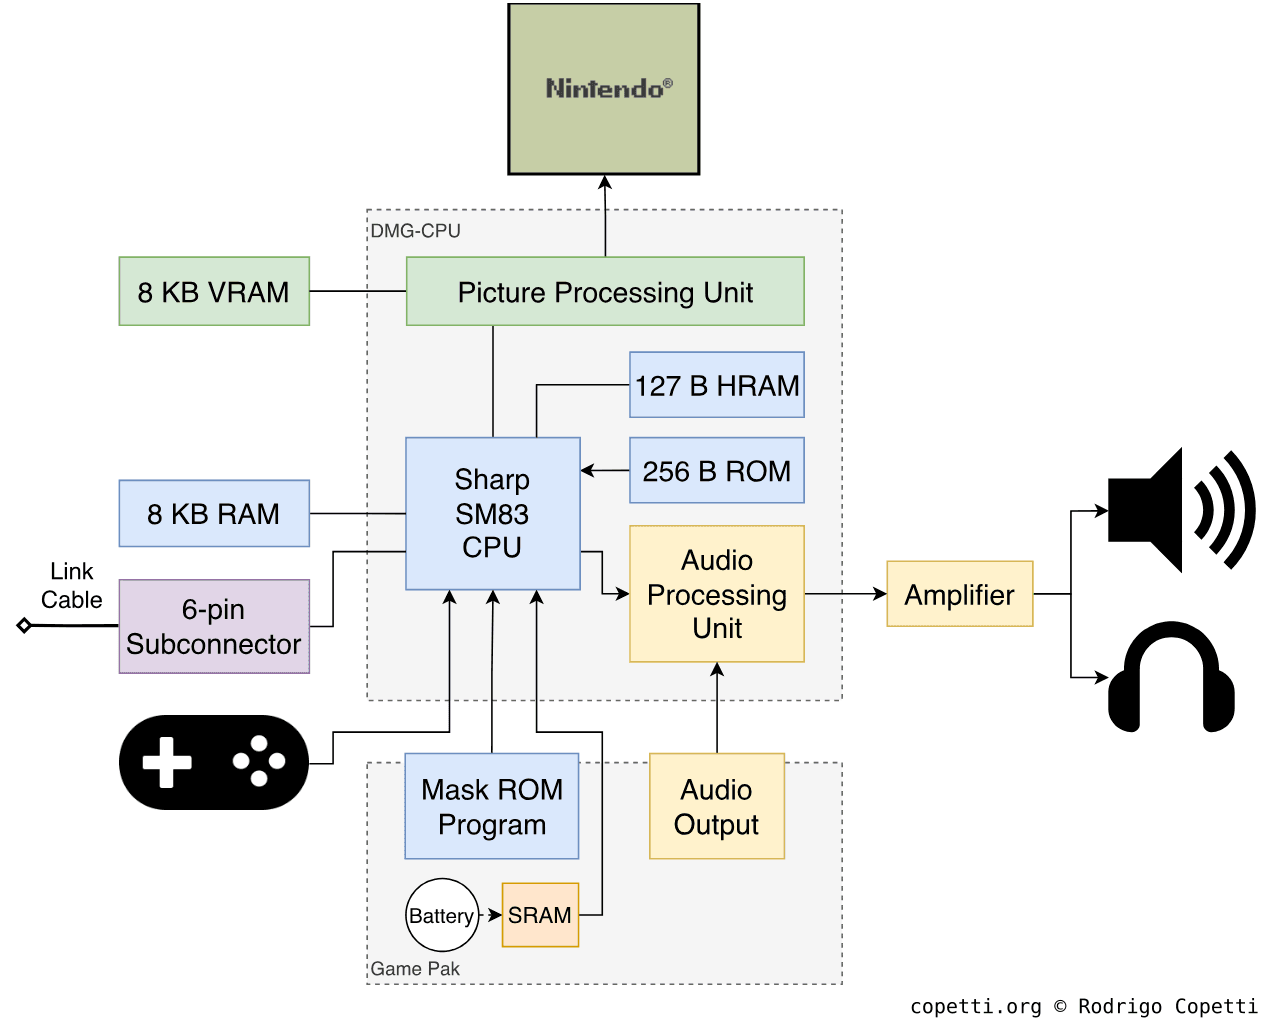
\includegraphics[width=0.60\textwidth]{imaxes/arch_diagram.png}
  \caption{Diagrama da arquitectura da Game Boy \cite{CopettiGameBoy}}
  \label{fig:diagrama-arch}
\end{figure}


\subsection{Buses e topoloxía}

A comunicación entre a \acrshort{cpu} e o resto de compoñentes realízase a través dun único bus de
datos de 8 bits e un bus de direccións de 16 bits, o que permite enderezar ata 64\,KiB
de espazo. Este espazo non está ocupado unicamente por memoria: nel mapéanse tamén os
rexistros de control dos diferentes periféricos, polo que un mesmo acceso de lectura ou
escritura pode dirixirse á \acrshort{ram}, á \acrshort{vram}, á \acrshort{rom} do cartucho ou a calquera rexistro de E/S
en función da dirección.


Por estar todos os compoñentes pendurados do mesmo bus, certos accesos entran en
conflito. O caso máis representativo é o acceso á \acrshort{vram} e á \acrshort{oam} por parte da \acrshort{ppu}: mentres
a \acrshort{ppu} está a debuxar unha liña, a \acrshort{cpu} non pode acceder a esas memorias e calquera
lectura devolve \texttt{0xFF}.

\section{Mapa de memoria}
\label{sec:mapa-memoria}

\begin{figure}[hp!]
  \centering
  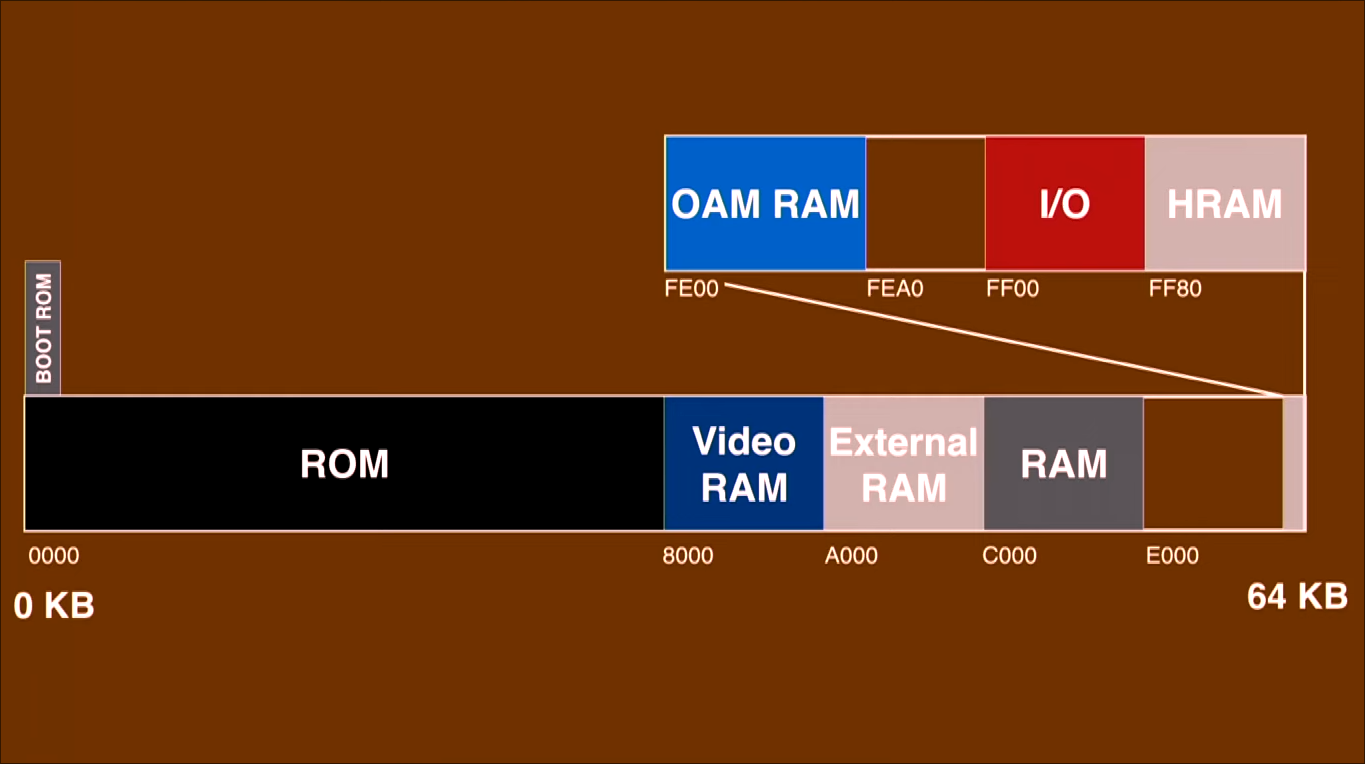
\includegraphics[width=0.60\textwidth]{imaxes/memory_map.png}
  \caption{Mapa de memoria da Game Boy \cite{UltimateGameBoyTalk}}
  \label{fig:memory-map}
\end{figure}


O espazo de 64\,KiB endereza\-ble non se corresponde cun único dispositivo de memoria,
senón que está dividido en rexións que o hardware redirixe ao compoñente adecuado
en función dos bits altos da dirección.
Cada espazo está asignado a diferentes compoñentes, como se amosa na figura~\ref{fig:memory-map}.

\subsection{Entrada/saída mapeada en memoria}

Para acceder aos periféricos, a consola emprega un esquema de entrada/saída mapeada en memoria.
Isto quere dicir que os rexistros comparten o mesmo espazo de direccións que a memoria principal.
Para manipular os periféricos, empréganse as mesmas instrucións de carga que para acceder á memoria,
e a súa dirección determina a que periférico se está a acceder.

Esta decisión simplifica o hardware, xa que evita duplicar lóxica de descodificación
e liñas de control, e explica varias das ausencias comentadas na
sección~\ref{subsec:comparativa-cpu}.

A seguinte táboa~\ref{tab:rexistros-io} recolle a súa distribución por periférico.

\begin{table}[htbp]
  \centering
  \rowcolors{2}{white}{udcgray!25}
  \begin{tabular}{l|l|>{\raggedright\arraybackslash}p{5.2cm}}
  \rowcolor{udcpink!25}
  \textbf{Rango} & \textbf{Periférico} & \textbf{Rexistros principais} \\\hline
  \texttt{0xFF00}       & Joypad        & \texttt{P1} (véxase sección~\ref{sec:joypad}). \\
  \texttt{0xFF01-0xFF02} & Serie         & \acrshort{sb}, \acrshort{sc}. \\
  \texttt{0xFF04-0xFF07} & Temporizador  & \acrshort{div}, \acrshort{tima}, \acrshort{tma}, \acrshort{tac}. \\
  \texttt{0xFF0F}       & Interrupcións & \acrshort{if}. \\
  \texttt{0xFF10-0xFF26} & \acrshort{apu} & Rexistros \texttt{NRxy} das catro canles e do mesturador. \\
  \texttt{0xFF30-0xFF3F} & \acrshort{apu} & \textit{Wave RAM}, a forma de onda da canle 3. \\
  \texttt{0xFF40-0xFF4B} & \acrshort{ppu} & \acrshort{lcdc}, \acrshort{stat}, \acrshort{dma}... \\
  \texttt{0xFF50}       & Boot \acrshort{rom} & Rexistro de desmapeo da Boot \acrshort{rom}. \\
  \end{tabular}
  \caption{Distribución dos rexistros de E/S mapeados en memoria~\cite{pandocs}.}
  \label{tab:rexistros-io}
\end{table}



\section{Unidade central de procesamento}
\label{sec:cpu}

A \acrshort{cpu} da consola é un procesador de 8 bits funcionando cun reloxo mestre de
4\,194\,304\,Hz, é dicir, $2^{22}$ oscilacións por segundo. Esa é a frecuencia que xera o
cristal do sistema, e cada unha das súas oscilacións coñécese como ciclo T
(\textit{T-cycle}).

Non todos os compoñentes do sistema funcionan a esta frecuencia. A memoria \acrshort{ram} funciona
a unha cuarta parte da frecuencia do procesador, é dicir, a 1\,048\,576\,Hz.
Debido a esta diferenza, todo o sistema está limitado pola memoria, de forma que
se fala de ciclos M (\textit{Machine cycle}) para referirse á unidade equivalente a catro ciclos T.

\begin{table}[htbp]
  \centering
  \rowcolors{2}{white}{udcgray!25}
  \begin{tabular}{l|c|l}
  \rowcolor{udcpink!25}
  \textbf{Compoñente} & \textbf{Frecuencia} & \textbf{Relación co reloxo mestre} \\\hline
  \acrshort{cpu} & 4\,MiHz & Reloxo mestre \\
  \acrshort{ppu} & 4\,MiHz & Reloxo mestre \\
  \acrshort{vram} & 2\,MiHz & Metade do reloxo mestre \\
  \acrshort{ram} & 1\,MiHz & Cuarta parte do reloxo mestre \\
  \end{tabular}
  \caption{Frecuencias de traballo dos principais compoñentes da consola}
  \label{tab:frecuencias}
\end{table}

A identidade exacta deste procesador foi durante moito tempo obxecto de confusión.
É habitual atopar referencias a este procesador como un Zilog Z80, que non se corresponde coa realidade.
Aínda que a súa sintaxe de ensamblador é de estilo Z80
e comparte con el unha parte do conxunto de instrucións,
trátase dun deseño propio de Sharp que está máis próximo ao Intel 8080,
como se detalla na sección~\ref{subsec:comparativa-cpu}.

Outra denominación máis correcta pero de igual forma incompleta é denominalo polo nome do
encapsulado completo, o Sharp LR35902.
O máis probable segundo a información dispoñible actualmente é que se trate dun Sharp SM83 \cite{sharpsm83}.

\begin{figure}[hp!]
  \centering
  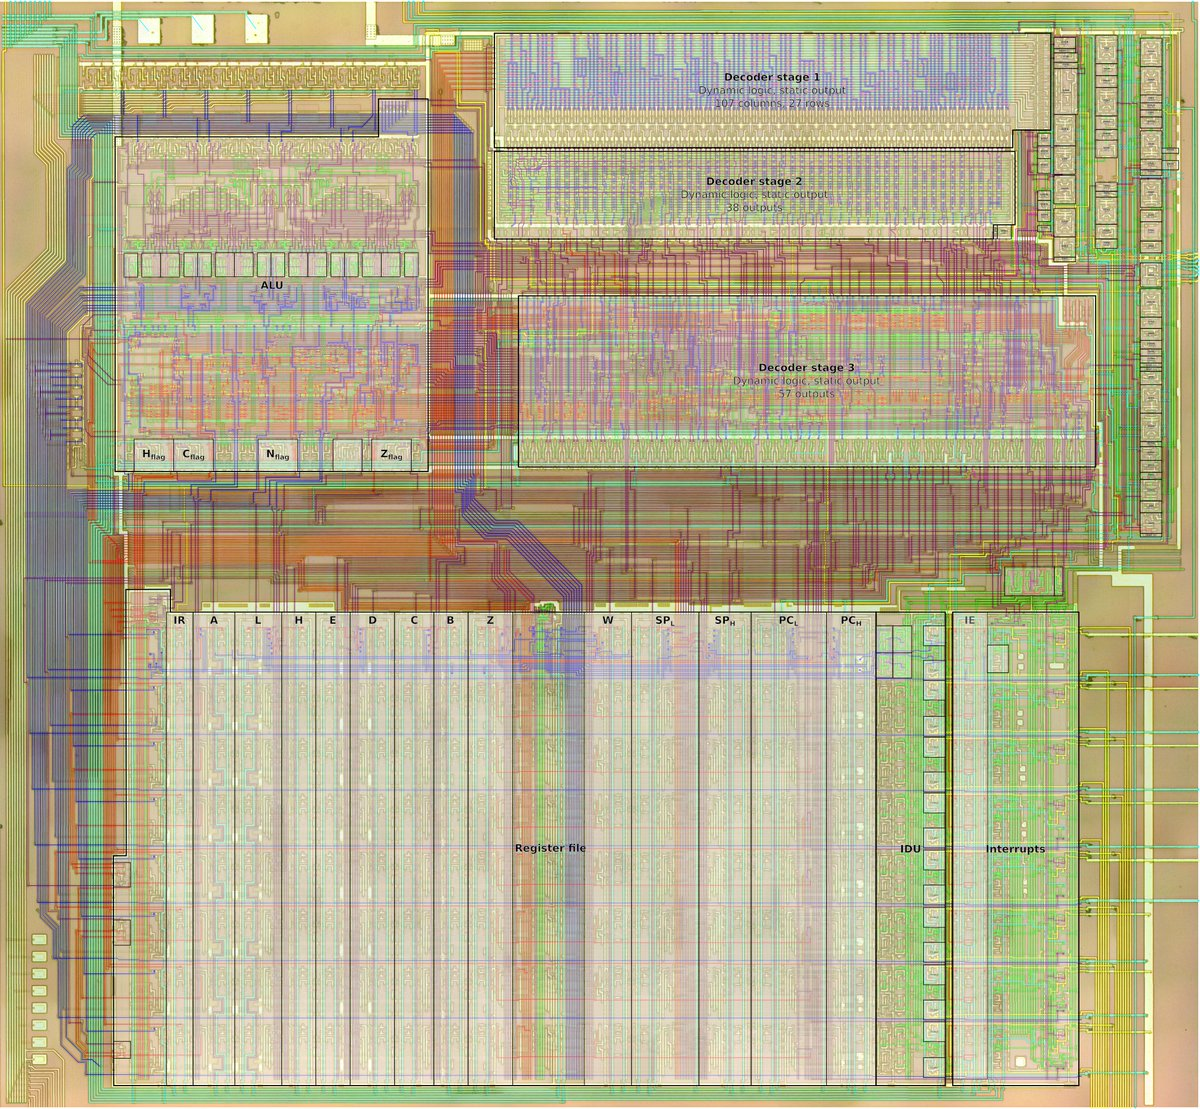
\includegraphics[width=0.85\textwidth]{imaxes/decap_sm83.jpg}
  \caption{Decapsulado do Sharp SM83}
  \label{fig:decap_sm83}
\end{figure}

\subsection{Conxunto de instrucións e rexistros}
\label{subsec:isa}

O SM83 conta cun banco de sete rexistros de propósito xeral de 8 bits,
o rexistro de \textit{flags},
máis dous rexistros de 16 bits de propósito específico.
Os rexistros de 8 bits pódense combinar por parellas para formar rexistros de 16 bits,
o que permite empregalos como punteiros dentro do espazo de direccións de 64\,KiB.
A táboa~\ref{tab:rexistros-cpu} recolle esta organización.

\begin{table}[htbp]
  \centering
  \rowcolors{2}{white}{udcgray!25}
  \setlength{\tabcolsep}{5pt}
  \begin{tabular}{c|c|c|l}
  \rowcolor{udcpink!25}
  \textbf{16 bits} & \textbf{Alto} & \textbf{Baixo} & \textbf{Función} \\\hline
  \texttt{AF} & \texttt{A} & \texttt{F} & Acumulador e rexistro de \textit{flags} \\
  \texttt{BC} & \texttt{B} & \texttt{C} & Propósito xeral \\
  \texttt{DE} & \texttt{D} & \texttt{E} & Propósito xeral \\
  \texttt{HL} & \texttt{H} & \texttt{L} & Propósito xeral e punteiro a memoria \\
  \texttt{SP} & --- & --- & Punteiro de pila (\textit{stack pointer}) \\
  \texttt{PC} & --- & --- & Contador de programa (\textit{program counter}) \\
  \end{tabular}
  \caption{Rexistros do procesador SM83~\cite{pandocs}.}
  \label{tab:rexistros-cpu}
\end{table}

O rexistro \texttt{A} é o acumulador, e sobre el operan practicamente todas as instrucións
aritméticas e lóxicas, que toman como segundo operando outro rexistro, un valor inmediato ou
o contido dunha posición de memoria.
O rexistro \texttt{F} non se pode empregar como operando das instrucións habituais de 8 bits,
aínda que si é accesible a través da parella \texttt{AF} coas instrucións \texttt{push} e \texttt{pop}.
O seu contido reflicte o resultado
da última operación executada mediante catro \textit{flags} situados no seu \gls{nibble} alto,
quedando o \gls{nibble} baixo sen empregarse.
A táboa~\ref{tab:flags-cpu} describe o seu significado.

\begin{table}[htbp]
  \centering
  \rowcolors{2}{white}{udcgray!25}
  \begin{tabular}{c|c|>{\raggedright\arraybackslash}p{9cm}}
  \rowcolor{udcpink!25}
  \textbf{Bit} & \textbf{Nome} & \textbf{Significado} \\\hline
  7 & \texttt{Z} & Activo se o resultado da operación é cero. \\
  6 & \texttt{N} & Activo se a última operación foi unha resta. \\
  5 & \texttt{H} & Acarreo do \gls{nibble} baixo ao alto. \\
  4 & \texttt{C} & Acarreo fóra do bit máis significativo, ou préstamo nunha resta. \\
  \end{tabular}
  \caption{\textit{Flags} do rexistro \texttt{F}~\cite{pandocs}.}
  \label{tab:flags-cpu}
\end{table}

Os \textit{flags} \texttt{Z} e \texttt{C} son os que empregan os saltos condicionais,
que aceptan as catro condicións \texttt{z}, \texttt{nz}, \texttt{c} e \texttt{nc}.
Os \textit{flags} \texttt{N} e \texttt{H}, en cambio, non son consultables directamente:
existen unicamente para dar servizo á instrución \texttt{daa},
que corrixe o resultado dunha suma ou resta para que sexa válido en representación
decimal codificada en binario (\acrshort{bcd}).

A parella \texttt{HL} recibe un tratamento especial dentro do conxunto de instrucións.
A codificación dos operandos de 8 bits reserva un dos oito valores posibles
para designar non un rexistro, senón o byte de memoria apuntado por \texttt{HL},
escrito \texttt{[hl]} na sintaxe de RGBDS.
Isto significa que calquera instrución que opere sobre un rexistro de 8 bits pode operar
tamén sobre memoria sen necesidade de opcodes adicionais, ao custo dun ciclo M extra
polo acceso ao bus. Este mecanismo converte a \texttt{HL} no punteiro de traballo habitual
dos programas.

Os dous rexistros restantes son de propósito específico.
O contador de programa \texttt{PC} contén a dirección da seguinte instrución a executar,
e o punteiro de pila \texttt{SP} apunta ao cume da pila,
empregada polas instrucións \texttt{push} e \texttt{pop} e polas chamadas a subrutinas.

\subsubsection{Codificación das instrucións}

O SM83 é un procesador \acrfull{cisc} de lonxitude de instrución variable:
cada instrución ocupa entre un e tres bytes, sendo o primeiro o \gls{opcode}
e os seguintes, se os houber, o operando inmediato de 8 ou 16 bits.
Existe ademais un prefixo, o byte \texttt{0xCB}, que dá acceso a un segundo
espazo de 256 opcodes adicados ás operacións de rotación, desprazamento
e manipulación de bits individuais. Do total de 256 opcodes sen prefixo, 11 non están asignados a ningunha instrución
e producen un bloqueo ao empregarse.

\begin{figure}[hp!]
  \centering
  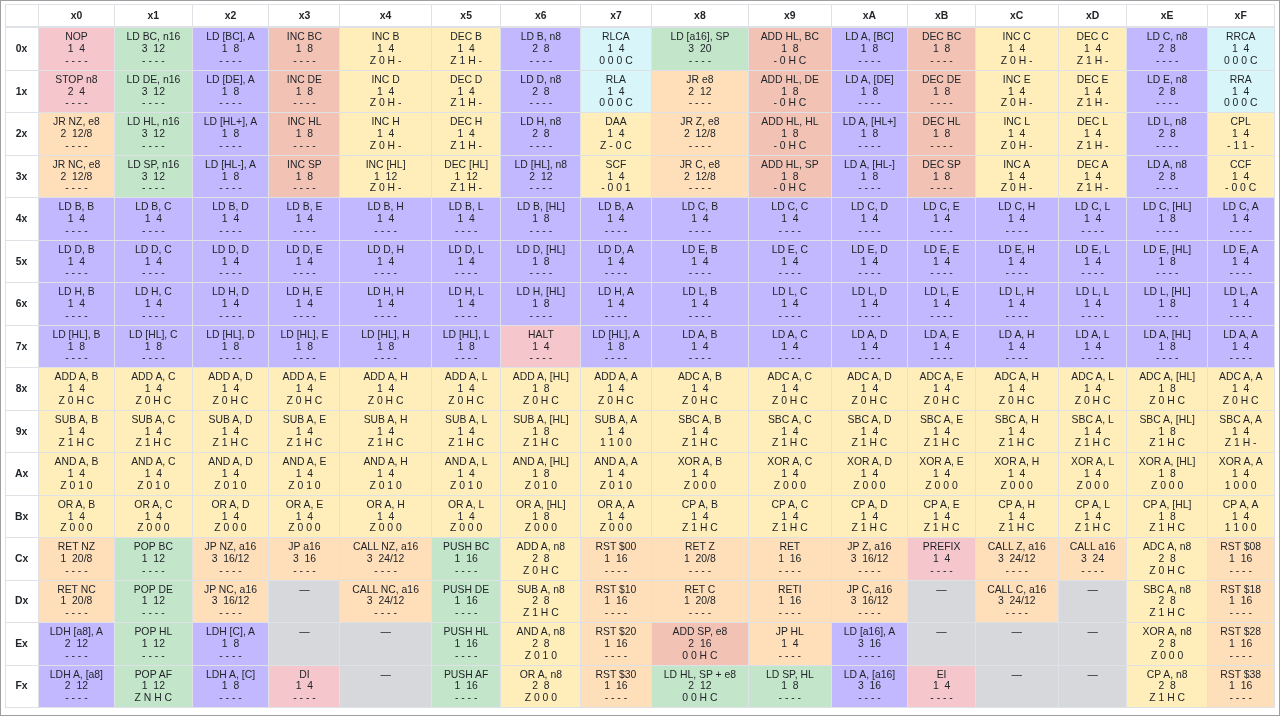
\includegraphics[width=0.85\textwidth]{imaxes/sm83_instruction_set.png}
  \caption{Conxunto de instrucións sen prefixo do SM83~\cite{pandocs}}
  \label{fig:sm83-instruction-set}
\end{figure}


O listado~\ref{lst:asm-exemplo} amosa un fragmento de código en ensamblador de RGBDS
que ilustra o uso destes mecanismos: unha rutina que copia un bloque de memoria
apoiándose en \texttt{HL} como punteiro de lectura autoincrementado.

\begin{lstlisting}[language={[x86masm]Assembler}, label={lst:asm-exemplo}]
; hl = orixe, de = destino, bc = numero de bytes a copiar
Copia:
  ; le [hl] no acumulador, incrementa hl e escribe o byte no destino
  ld a, [hl+]   
  ld [de], a    
  ; incrementamos os contadores
  inc de
  dec bc
  ld a, b
  ; comproba se bc chegou a cero
  or a, c
  ; salto relativo de un byte
  jr nz, Copia  
  ret
\end{lstlisting}


\subsection{Comparativa co Intel 8080 e o Zilog Z80}
\label{subsec:comparativa-cpu}

Mentres que o conxunto de instrucións do Zilog Z80 é un superconxunto do Intel 8080,
o SM83 soporta as características principais do Intel 8080, algunhas características do Z80,
como son os saltos relativos \texttt{jr} e a instrución \texttt{reti},
e engade algunhas instrucións propias como \texttt{ldh} e \texttt{swap}.

\begin{figure}[hp!]
  \centering
  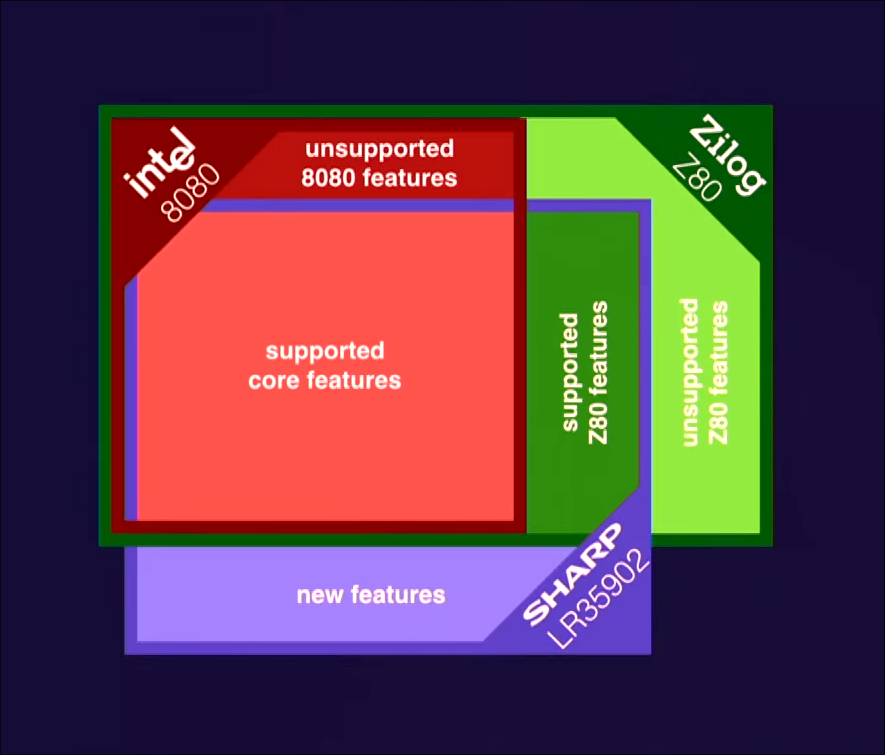
\includegraphics[width=0.50\textwidth]{imaxes/cpu_comparation.png}
  \caption{Comparativa da \acrshort{cpu} \cite{UltimateGameBoyTalk}}
  \label{fig:cpu-comparation}
\end{figure}

Do Intel 8080 non herda dúas bandeiras de estado, a de signo e a de paridade,
e polo tanto tampouco as emprega como condicións nas instrucións de salto.
Ademáis, tampouco soporta as instrucións de entrada/saída dedicadas \texttt{in} e \texttt{out},
xa que como se comenta na sección~\ref{sec:mapa-memoria}, os periféricos da consola
están mapeados en memoria e o seu acceso realízase coas mesmas instrucións de carga
empregadas para acceder ao resto do espazo de direccións.

O que non herda do Z80 é moito máis amplo.
Non existe o segundo banco de rexistros nin, en consecuencia, as instrucións
de intercambio entre bancos, nin os rexistros de índice \texttt{IX} e \texttt{IY}
cos seus prefixos \texttt{0xDD} e \texttt{0xFD}.
Desaparece por completo o espazo prefixado con \texttt{0xED},
o que elimina os accesos a memoria de 16 bits, boa parte da aritmética de 16 bits
e as instrucións de bloque que o Z80 empregaba para copiar rexións de memoria
nunha soa instrución.

Fronte estas ausencias, o SM83 engade instrucións propias que responden
directamente ás necesidades da consola.
As máis características son as cargas con post-incremento e post-decremento
de \texttt{HL} (\texttt{ld a, [hl+]} e \texttt{ld a, [hl-]}, e as súas versións de escritura),
que combinan nunha única instrución o acceso a memoria e a actualización do punteiro.
A segunda achega característica é o acceso rápido á páxina alta do espazo de direccións
mediante as instrucións \texttt{ldh}, que toman un operando de 8 bits
e o interpretan como un desprazamento sobre \texttt{0xFF00}.
Como xa se comentou na sección~\ref{sec:mapa-memoria}, nestes últimos 256 bytes da memoria
atópanse rexistros de E/S e a \acrshort{hram}, polo que resulta moi beneficioso ter un 
acceso máis eficiente a estas zonas.

Estas instrucións aforran un byte e un ciclo M en cada acceso fronte á carga absoluta
de 16 bits equivalente.
Complétanse cunha variante que toma o desprazamento do rexistro \texttt{C},
substituíndo as instrucións \texttt{in} e \texttt{out} eliminadas,
e con outras adicións menores como \texttt{swap}, que intercambia os dous \glspl{nibble} dun rexistro,
ou \texttt{stop}, que activa o modo de baixo consumo da consola.


\subsection{Interrupcións}
\label{subsec:interrupcions}

A consola dispón de cinco fontes de interrupción, unha por cada periférico
capaz de reclamar a atención do procesador.
O seu mecanismo de atención é notablemente máis simple que o dos procesadores modernos,
e herda directamente a filosofía do 8080.

Non existe unha táboa de vectores de interrupción propiamente dita.
Nun esquema vectorizado convencional, o procesador consulta unha táboa en memoria
para obter a dirección do manexador correspondente, o que permite reubicar
os manexadores libremente. No SM83, en cambio, cada interrupción ten asociada
unha dirección fixa no comezo do espazo de direccións, separadas oito bytes entre si,
á que o procesador salta directamente.
Esas oito posicións son, na práctica, o espazo dispoñible para o manexador,
polo que os programas adoitan colocar nelas unicamente un salto
á rutina real situada noutro punto da \acrshort{rom}.
A táboa~\ref{tab:interrupcions} recolle as cinco interrupcións, o seu vector e a súa orixe.

\begin{table}[htbp]
  \centering
  \rowcolors{2}{white}{udcgray!25}
  \begin{tabular}{c|l|c|p{5cm}}
  \rowcolor{udcpink!25}
  \textbf{Bit} & \textbf{Fonte} & \textbf{Vector} & \textbf{Condición de activación} \\\hline
  0 & VBlank      & \texttt{0x0040} & A \acrshort{ppu} entra no período de borrado vertical. \\
  1 & LCD (STAT)  & \texttt{0x0048} & A \acrshort{ppu} chega a unha condición configurada no rexistro \texttt{STAT}. \\
  2 & Timer       & \texttt{0x0050} & O rexistro contador do temporizador desborda. \\
  3 & Serial      & \texttt{0x0058} & Complétase unha transferencia de 8 bits polo porto serie. \\
  4 & Joypad      & \texttt{0x0060} & Algún dos bits 0--3 do rexistro \texttt{P1} pasa de alto a baixo. \\
  \end{tabular}
  \caption{Fontes de interrupción da consola, ordenadas de maior a menor prioridade~\cite{pandocs}.}
  \label{tab:interrupcions}
\end{table}

O mesmo principio de direccións fixas aplícase ás interrupcións software,
que se solicitan coa instrución \texttt{rst}.
Esta instrución, herdada tamén do 8080, realiza unha chamada a subrutina
a unha das oito direccións fixas comprendidas entre \texttt{0x0000} e \texttt{0x0038},
codificando o destino nos propios bits do opcode.
Ao ocupar un só byte fronte aos tres da chamada convencional \texttt{call},
os xogos empregan estas posicións como puntos de entrada ás rutinas máis frecuentes,
aforrando espazo na \acrshort{rom}.
Isto explica a distribución da primeira parte do mapa de memoria:
os primeiros 256 bytes da \acrshort{rom} do cartucho están reservados
para os destinos de \texttt{rst}, os vectores de interrupción e a cabeceira.

O control das interrupcións repártese entre tres elementos.
Os rexistros \acrshort{ie} (mapeado en \texttt{0xFFFF})
e \acrfull{if} (mapeado en \texttt{0xFF0F}) empregan os seus cinco bits baixos
seguindo a orde da táboa~\ref{tab:interrupcions}:
\acrshort{ie} indica que interrupcións están habilitadas
e \acrshort{if} cales están pendentes de atender.
Cando un periférico solicita atención, o hardware activa o bit correspondente de \acrshort{if}
de forma automática, aínda que o programa tamén pode escribir neste rexistro
para solicitar ou descartar interrupcións manualmente.
A conxunción \acrshort{ie}\,\&\,\acrshort{if} determina, polo tanto, que interrupcións
están en condicións de ser atendidas.

Por riba destes dous rexistros sitúase o \textit{flag} \acrfull{ime},
interno ao procesador e non accesible en memoria,
que habilita ou deshabilita globalmente a atención de interrupcións.
Actívase coa instrución \texttt{ei} e desactívase con \texttt{di},
e o propio procesador ponno a cero ao atender unha interrupción,
evitando o aniñamento agás que o manexador o habilite explicitamente.

Cando \acrshort{ime} está activo e \acrshort{ie}\,\&\,\acrshort{if} é distinto de cero,
o procesador borra o bit correspondente de \acrshort{if}, pon \acrshort{ime} a cero
e realiza unha chamada ao vector correspondente,
apilando o valor actual do \texttt{PC}.
Todo o proceso consome cinco ciclos M: dous de espera, dous para apilar o \texttt{PC}
e un último para cargar a dirección do vector.

A prioridade entre interrupcións simultáneas é fixa e vén dada pola orde dos bits
en \acrshort{ie} e \acrshort{if}: o bit 0 (VBlank) ten a prioridade máis alta
e o bit 4 (Joypad) a máis baixa.

\section{Unidade de procesamento de píxeles}
\label{sec:ppu}

A \acrshort{ppu} é o compoñente encargado de xerar a imaxe que se amosa na pantalla
de cristal líquido da consola, de 160$\times$144 píxeles e catro tonalidades de gris.
A diferenza dunha \acrshort{gpu} moderna, non existe un búfer de imaxe completo en memoria:
a \acrshort{ppu} constrúe a imaxe liña a liña e en tempo real,
tomando os datos da \acrshort{vram} e da \acrshort{oam}.

A imaxe non se describe píxel a píxel, senón mediante \glspl{tile}, bloques de
8$\times$8 píxeles almacenados na \acrshort{vram}. Cada fila dun \gls{tile} ocúpase
con dous bytes, de forma que ocupa un enteiro 16 bytes, 
que actúan como planos de bits. Os bits da mesma posición en ambos
os dous bytes combínanse para formar o valor de dous bits dese píxel.

Ese valor de dous bits non é unha cor directa, senón un índice dentro dunha paleta,
o que permite alterar o aspecto de toda a pantalla modificando un único rexistro.
Isto emprégase para diversos efectos visuais cun custo moi baixo, xa que non
require substituír os datos de cada \gls{tile}.

\begin{figure}[hp!]
  \centering
  \begin{subfigure}[c]{0.35\textwidth}
    
\includegraphics[width=\textwidth]{imaxes/palette_normal.png}
    \caption{Paleta normal}
    \label{fig:palette-normal}
  \end{subfigure}
  \hspace{0.02\textwidth}
  \begin{subfigure}[c]{0.35\textwidth}
    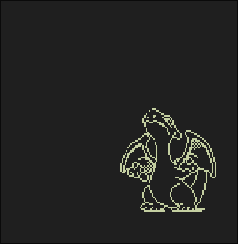
\includegraphics[width=\textwidth]{imaxes/palette_reversed.png}
    \caption{Paleta invertida}
    \label{fig:palette-reversed}
  \end{subfigure}
  \caption{Exemplo do cambio de paleta mediante o rexistro \texttt{BGP}~\cite{pandocs}.}
  \label{fig:palette-switch-example}
\end{figure}


\subsection{Modos de funcionamento}
\label{subsec:ppu-modos}

A unidade mínima de tempo da \acrshort{ppu} é o \textit{dot}, equivalente a un ciclo T.
Para a construción de cada liña da pantalla consúmense 456 \textit{dots} e un cadro completo comprende 154 liñas,
das cales só as 144 primeiras son visibles. Isto dá un total de 70\,224 \textit{dots}
por cadro e unha frecuencia de refresco de aproximadamente 59,7\,Hz.

Ao longo dese percorrido, a \acrshort{ppu} vai alternando entre diferentes modos de
funcionamento, que se poden consultar nos dous bits baixos do rexistro \texttt{STAT}
e que determinan, ademais, a accesibilidade da \acrshort{vram} e da \acrshort{oam} por parte
da \acrshort{cpu}. A seguinte táboa~\ref{tab:ppu-modos} recolle os catro modos.

\begin{table}[htbp]
  \centering
  \rowcolors{2}{white}{udcgray!25}
  \begin{tabular}{c|l|c|>{\raggedright\arraybackslash}p{2.3cm}}
  \rowcolor{udcpink!25}
  \textbf{Modo} & \textbf{Nome} & \textbf{Duración} & \textbf{Acceso bloqueado} \\\hline
  2 & Busca en \acrshort{oam} & 80 \textit{dots}      & \acrshort{oam} \\
  3 & Transferencia de píxeles & 172--289 \textit{dots} & \acrshort{oam} e \acrshort{vram} \\
  0 & \textit{HBlank}          & 87--204 \textit{dots}  & Ningún \\
  1 & \textit{VBlank}          & 4560 \textit{dots}     & Ningún \\
  \end{tabular}
  \caption{Modos de funcionamento da \acrshort{ppu}~\cite{pandocs}.}
  \label{tab:ppu-modos}
\end{table}

Durante o modo 2 a \acrshort{ppu} percorre as 40 entradas da \acrshort{oam} para determinar
cales dos obxectos son visibles na liña actual, seleccionando como máximo dez deles.
No modo 3 emítense os píxeles á pantalla, combinando o fondo, a xanela e os obxectos
seleccionados. A súa duración non é fixa: increméntase co desprazamento fino do
fondo e co número de obxectos presentes na liña, e o tempo que se alonga réstase do modo 0
seguinte, de forma que a suma dos tres modos por liña permanece constante en 456 \textit{dots}.

Rematadas as 144 liñas visibles, a \acrshort{ppu} entra no modo 1 durante dez liñas
adicionais e solicita a interrupción \textit{VBlank} descrita na
táboa~\ref{tab:interrupcions}. Este é o único intervalo no que a \acrshort{vram} e a
\acrshort{oam} están accesibles durante un tempo prolongado, polo que os xogos concentran
nel todas as actualizacións gráficas.
A alternativa para modificar a \acrshort{oam} é a transferencia \acrfull{dma}.
Consiste na copia automática de 160 bytes desde calquera páxina de memoria
á \acrshort{oam} en 160 ciclos M, sen intervención do procesador, a través da escritura
no rexistro mapeado en \texttt{0xFF46}. Durante este tempo, a \acrshort{cpu} só pode
acceder a \acrshort{hram}, polo que o recomendado e iniciar esta transferencia dende
código residente na \acrshort{hram}, onde o programa debe empezar e acabar a transferencia para evadir
o conflito no bus.

O rexistro \texttt{STAT} permite ademais configurar unha segunda fonte de interrupción,
programable para dispararse ao entrar nos modos 0, 1 ou 2, ou ben cando o contador de liña
\texttt{LY} coincide co valor escrito en \texttt{LYC}. Esta última condición é a base dos
efectos gráficos por liña característicos da plataforma, que se conseguen modificando os
rexistros de desprazamento xusto antes de que se debuxe unha liña concreta.

\subsection{Fondo, xanela e obxectos}
\label{subsec:ppu-capas}

A imaxe final resulta da superposición de tres capas, cuxa habilitación e configuración
se controlan desde o rexistro \acrfull{lcdc}.

O fondo (\textit{background}) é unha superficie de 256$\times$256 píxeles, descrita
por un mapa de 32$\times$32 bytes na \acrshort{vram} no que cada byte é o índice do
\gls{tile} que ocupa esa posición. Existen dous mapas dispoñibles, situados en
\texttt{0x9800} e \texttt{0x9C00}, e cada capa escolle o que vai empregar mediante un bit
de \acrshort{lcdc}, o que permite construír un mapa completo mentres se amosa o outro.

O que vemos pola pantalla é un \gls{viewport} sobre este fondo
cuxa esquina superior esquerda vén dada polos rexistros de desprazamento \texttt{SCX} e \texttt{SCY}.
Modificar estes dous rexistros despraza todo o fondo sen tocar
a \acrshort{vram}, permitindo crear efectos de desprazamento como podemos ver
na figura~\ref{fig:vram-oam-representation}. 

A xanela (\textit{window}) é unha segunda capa de fondo, opaca e sen desprazamento
propio, que se debuxa por riba do fondo a partir da posición indicada polos rexistros
\texttt{WX} e \texttt{WY}. Emprégase habitualmente para amosar información fixa que non debe verse
afectada polo desprazamento do escenario, como marcadores de estado ou caixas de diálogo.

Os obxectos (\textit{objects} na nomenclatura de Nintendo, aínda que habitualmente chamados \textit{sprites})
son os elementos móbiles da imaxe.
Poden medir 8$\times$8 ou 8$\times$16 píxeles, dependendo da configuración do rexistro \acrshort{lcdc},
e dispoñen dunha cor transparente, o índice cero da súa paleta, que deixa ver a capa
inferior.
Cada un descríbese mediante unha entrada de catro bytes na \acrshort{oam}, cuxo contido
se recolle na táboa~\ref{tab:oam-entrada}.

\begin{table}[htbp]
  \centering
  \begin{tabular}{l|c|>{\raggedright\arraybackslash}p{6.5cm}}
  \rowcolor{udcpink!25}
  \textbf{Atributo} & \multicolumn{2}{c}{\textbf{Descrición}} \\\hline
  \rowcolor{udcgray!25}
  \textit{Coordenada Y} & \multicolumn{2}{l}{Posición vertical, desprazada 16 píxeles.} \\
  \textit{Coordenada X} & \multicolumn{2}{l}{Posición horizontal, desprazada 8 píxeles.} \\
  \rowcolor{udcgray!25}
  \textit{Índice}       & \multicolumn{2}{l}{\Gls{tile} que representa o obxecto.} \\\hline
  \multirow{6}{*}{\textit{Atributos}} & \textbf{Bit} & \\
                        & \cellcolor{udcgray!25} 7    & \cellcolor{udcgray!25} Indica se as cores 1-3 do fondo ou da xanela teñen que ter prioridade sobre o obxecto. \\
                        & 6                           & Reflexión vertical, sobre o eixo X. \\
                        & \cellcolor{udcgray!25} 5    & \cellcolor{udcgray!25} Reflexión horizontal, sobre o eixo Y. \\
                        & 4                           & Indica se se emprega a paleta \texttt{OBP0} ou a \texttt{OBP1}. \\
                        & \cellcolor{udcgray!25} 3--0 & \cellcolor{udcgray!25} Sen uso na \acrshort{dmg}. \\
  \end{tabular}
  \caption{Atributos dun obxecto na súa entrada da \acrshort{oam}~\cite{pandocs}.}
  \label{tab:oam-entrada}
\end{table}


Ese desprazamento das coordenadas permite que un obxecto entre e saia da pantalla
parcialmente polos bordos superior e esquerdo, xa que a posición cero equivale a estar
completamente fóra.
As estritas limitacións do hardware só fai posible debuxar dez
obxectos por liña, e os que exceden ese límite simplemente desaparecen.
Cando dous se solapan, ten prioridade o de coordenada X menor e, en caso de empate,
o que ocupe unha posición máis baixa na \acrshort{oam}.

As tres capas comparten un espazo de \glspl{tile} de 384 entradas, situado entre
\texttt{0x8000} e \texttt{0x97FF} e dividido en tres bloques de 128.
Os obxectos direccionan sempre
os dous primeiros bloques cun índice sen signo a partir de \texttt{0x8000}, mentres que o
fondo e a xanela poden empregar ese mesmo método ou ben un direccionamento con signo a
partir de \texttt{0x9000}, seleccionable mediante un bit de \acrshort{lcdc}, o que permite
que ambas as capas compartan o bloque central.

O algoritmo que está detrás da composición destas tres capas é o chamado \textit{pixel FIFO}~\cite{pandocs}.
Durante o modo 3 da \acrshort{ppu}, esta mantén dúas colas independentes de ata dezaseis píxeles,
unha para o fondo e a xanela e outra para os obxectos,
alimentadas por unha unidade de busca (\textit{fetcher}) que traballa por filas completas de oito píxeles.

\begin{enumerate}
  \item obtén o índice do \gls{tile} no mapa correspondente,
  \item le o primeiro byte da fila que lle toca a esa liña,
  \item le o segundo byte, co que xa dispón dos oito píxeles completos,
  \item agarda sen facer traballo ningún,
  \item e insire os oito píxeles na cola, o que só é posible cando esta quedou baleira.
\end{enumerate}

En paralelo, por cada \textit{dot} extráese un píxel de cada cola e mestúranse 
de forma que prevalece o do obxecto agás que sexa transparente ou dunha prioridade menor.
Só entón se traduce o índice resultante a través da paleta correspondente
e o píxel final se debuxa na pantalla.

Este deseño explica que a duración do modo 3 non sexa fixa. O desprazamento fino do fondo
obriga a descartar os primeiros \texttt{SCX} $\bmod$ 8 píxeles xa producidos, a aparición
da xanela baleira a cola de fondo e reinicia o \textit{fetcher}, e cada obxecto presente na
liña interrompe a busca en curso para intercalar a súa propia. Cada unha destas situacións
engade \textit{dots} ao modo 3 que se restan do \textit{HBlank} seguinte, de aí os rangos
recollidos na táboa~\ref{tab:ppu-modos}.

A figura~\ref{fig:ppu-composition-vram-oam} ilustra esta organización cun cadro real.


\begin{figure}[hp!]
  \centering
  \begin{subfigure}[c]{0.50\textwidth}
    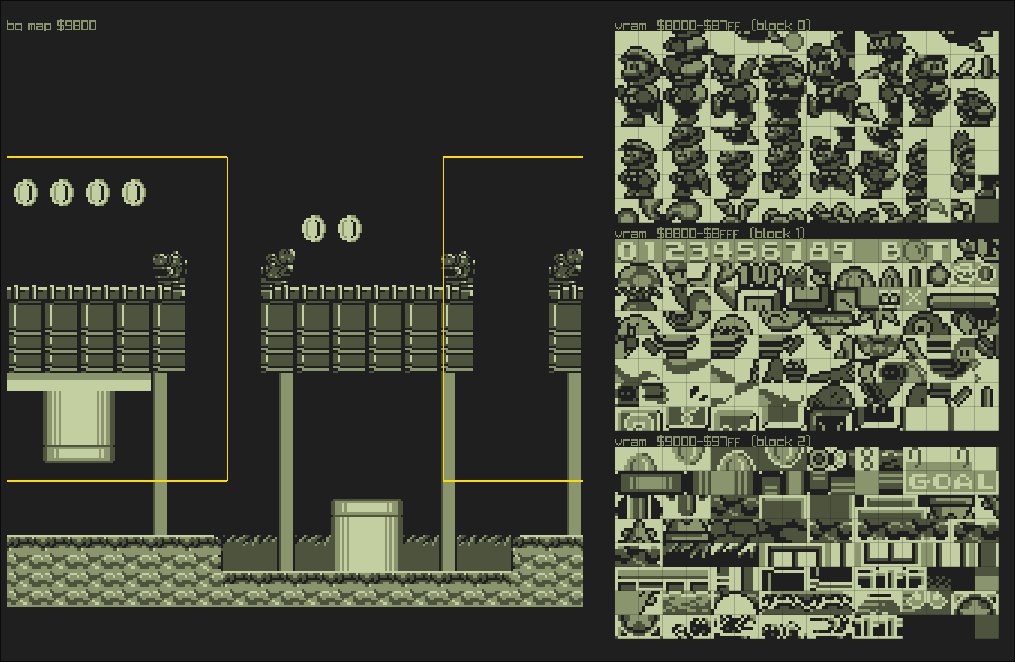
\includegraphics[width=\textwidth]{imaxes/vram_oam_representation.png}
    \caption{Mapa de fondo, coa área visible marcada, e os tres bloques de \glspl{tile} da \acrshort{vram}.}
    \label{fig:vram-oam-representation}
  \end{subfigure}
  \hspace{0.02\textwidth}
  \begin{subfigure}[c]{0.40\textwidth}
    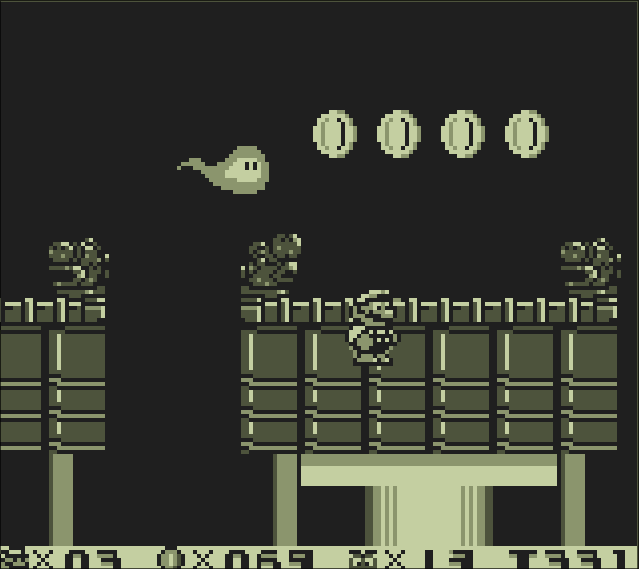
\includegraphics[width=\textwidth]{imaxes/ppu_composition.png}
    \caption{Cadro final, coas tres capas xa compostas.}
    \label{fig:ppu-composition}
  \end{subfigure}
  \caption{Composición dun cadro a partir dos datos da \acrshort{vram} e da \acrshort{oam}.}
  \label{fig:ppu-composition-vram-oam}
\end{figure}

\section{Cartuchos}
\label{sec:cartuchos}

Os cartuchos non forman parte do hardware da consola propiamente dita, pero teñen unha
importancia capital no seu funcionamento. A súa función non se limita a proporcionar os
datos e o código do xogo: son tamén o mecanismo mediante o cal a consola foi capaz de
estender as súas capacidades ao longo de toda a súa vida comercial, incorporando memoria
adicional, almacenamento persistente grazas a pilas e mesmo periféricos completos.

Por exemplo, os cartuchos iniciais, máis sinxelos, soamente contiñan 32\,KiB de datos na súa ROM,
que era todo o que podía direccionar a consola directamente. Co hardware adicional dos \acrshort{mbc},
podíanse empregar \acrshort{rom} de ata 8\,MiB.

Movendo o custo e a ampliación das capacidades da consola ao cartucho, Nintendo conseguiu
que as consolas xa vendidas puidesen executar xogos moito máis esixentes sen modificación ningunha.

\subsection{ROM e arranque}

Como xa se comentou na sección~\ref{sec:vision-xeral}, ao acender a consola o procesador
non executa código do cartucho, senón a Boot \acrshort{rom}, que se superpón aos primeiros
256 bytes do espazo de direccións.
Rematadas as súas comprobacións e inicializacións, esta debe cederlle o control ao cartucho, e faino
escribindo un valor distinto de cero no rexistro \texttt{0xFF50}, o que provoca que o
hardware a desmapee permanentemente e deixe visible a \acrshort{rom} do cartucho nese rango.

\begin{lstlisting}[language={[x86masm]Assembler}, label={lst:bootrom-unmap}]
  ; últimas instrucións da Boot ROM
  ld a, $01
  ldh [$50], a

  ; primeiras instrucións de calquera cartucho,
  ; saltando ata despois da cabeceira
  nop
  jp $0150

\end{lstlisting}

Ao completarse a instrución, o contador de programa
xa apunta á dirección \texttt{0x0100} do cartucho.

Ese punto de entrada dispón unicamente de catro bytes antes da cabeceira, polo que se
limita a saltar co \texttt{jp} ata o código de inicio real situado tras ela.

\subsubsection{Cabeceira do cartucho}

Os primeiros 336 bytes da \acrshort{rom} teñen unha estrutura fixa.
Os 256 primeiros, como se explicou na sección~\ref{subsec:interrupcions}, están ocupados
polos destinos de \texttt{rst} e polos vectores de interrupción; a continuación, entre
\texttt{0x0104} e \texttt{0x014F}, sitúase a cabeceira, un bloque de metadatos que describe
o propio cartucho.

Podemos atopar información como o nome e fabricante do xogo, a súa compatibilidade con diferentes
modelos como a \acrfull{sgb} e a \acrfull{gbc}, o tipo de cartucho, co que coñecemos o
hardware que incorpora o cartucho; o tamaño das memorias e sumas de control
(tanto da cabeceira como de toda a \acrshort{rom}) para verificar a integridade dos datos.

Os datos do tamaño das memorias non son empregados pola consola, pero para a implementación dun emulador son 
esenciais para coñecer o tipo de cartucho, e a si ser capaz de emulalo correctamente, e reservar a suficiente memoria
para a \acrshort{rom} e a \acrshort{ram} externa.

\subsection{Controladores de bancos de memoria}
\label{sec:mbc}

O \acrshort{mbc} é un circuíto integrado situado no propio cartucho que se interpón entre
o bus de direccións da consola e os chips de memoria.
A súa función é a conmutación de bancos: presentar, nunha mesma xanela do mapa de memoria,
fragmentos distintos dunha memoria moito maior que o espazo direccionable.

O mecanismo apóiase nunha particularidade do bus: a \acrshort{rom} do cartucho é de só
lectura, polo que o banco aproveita esas escrituras como canle de control, almacenando o dato nun
rexistro interno que determina que banco queda visible na xanela conmutable.
Cada tipo de cartucho emprega rexistros distintos agrupados en varios grupos principais,
que aínda así poden conter diferente hardware adicional, como baterías, \acrfull{rtc}
ou motores de vibración.
O byte \texttt{0x0147} da cabeceira non identifica só a familia de controlador,
senón a combinación exacta de compoñentes que leva o cartucho, de xeito que un mesmo
\acrshort{mbc} dá lugar a varias variantes, cada unha cunha capacidade de \acrshort{rom}
e de \acrshort{ram} distinta; a táboa~\ref{tab:mbc} recolle as familias máis
empregadas e o hardware que poden incorporar.


\begin{table}[htbp]
  \centering
  \rowcolors{2}{white}{udcgray!25}
  \begin{tabular}{l|c|c|>{\raggedright\arraybackslash}p{3.6cm}}
  \rowcolor{udcpink!25}
  \textbf{Familia} & \textbf{\acrshort{rom} máx.} & \textbf{\acrshort{ram} máx.} & \textbf{Hardware adicional} \\\hline
  Ningunha & 32\,KiB & 8\,KiB & \acrshort{ram} e batería \\
  MBC1 & 2\,MiB & 32\,KiB & \acrshort{ram} e batería \\
  MBC2 & 256\,KiB & 512$\times$4 bits & Batería; a \acrshort{ram} vai integrada no controlador \\
  MBC3 & 2\,MiB & 32\,KiB & \acrshort{ram}, batería e \acrshort{rtc} \\
  MBC5 & 8\,MiB & 128\,KiB & \acrshort{ram}, batería e vibración \\
  Outras & --- & --- & MBC6, MBC7, MMM01, HuC1, HuC3 e Pocket Camera \\
  \end{tabular}
  \caption{Familias de controladores de bancos de memoria, coas capacidades máximas que admiten e o hardware que poden incorporar~\cite{pandocs}.}
  \label{tab:mbc}
\end{table}

\subsection{Hardware adicional implementado nos cartuchos}

Unha vez establecido o cartucho como punto de extensión do sistema, os fabricantes
aproveitárono para incorporar hardware que vai moito máis alá da memoria.
O engadido máis estendido é a batería empregada para ter memoria persistente.
A \acrshort{ram} externa é volátil, polo que os
cartuchos que precisan gardar a partida inclúen unha pila de botón que a mantén alimentada
mentres a consola está apagada, e a súa descarga trinta anos despois é a causa habitual de
que os cartuchos orixinais perdan as partidas gardadas.
Sobre esa mesma alimentación permanente constrúese o \acrshort{rtc} dos MBC3, un contador de
tempo real que segue avanzando coa consola apagada e que permite implementar ciclos de día
e noite ou eventos dependentes da data.

Outros cartuchos foron aínda máis lonxe: o MBC5 permite controlar un motor de vibración,
o MBC7 incorpora un acelerómetro de dous eixos empregado como sistema de control por
inclinación, e a Game Boy Camera integra directamente un sensor de imaxe no cartucho
xunto coa lóxica necesaria para capturar e procesar fotografías.
En todos estes casos o mecanismo é o mesmo, o periférico exponse como un conxunto de
rexistros accesibles desde o espazo de direccións do cartucho, sen que a consola precise
saber nada del.


\section{Joypad}
\label{sec:joypad}

A consola conta con oito botóns: a cruceta direccional, os botóns de acción \textit{A} e \textit{B},
e os botóns \textit{Start} e \textit{Select}.

Para representar estes oito botóns empréganse soamente seis bits mapeados na dirección de memoria \texttt{0xFF00},
no rexistro denominado \texttt{P1} ou \texttt{JOYP}.
Deste xeito o \acrshort{soc} pódese aforrar dúas liñas para conectar estes botóns.
Esta matriz de dúas columnas e catro filas permite codificar o estado dos oito botóns usando dous destes bits
como selectores. Estes bits selectores determinan cal das dúas columnas se vai ler, e os catro bits restantes devolven o estado dos botóns da columna seleccionada.
Cando se escribe un cero nun destes bits selectores, a columna correspondente queda seleccionada e os catro bits restantes devolven o estado dos botóns da columna seleccionada.


\begin{table}[htbp]
  \centering
  \rowcolors{2}{white}{udcgray!25}
  \begin{tabular}{c|l|l|l}
  \rowcolor{udcpink!25}
  \textbf{Bit} & \textbf{Función} & \textbf{Botóns} & \textbf{Direccións} \\\hline
  5 & Selección de botóns de acción & \multicolumn{2}{c}{0 selecciona esta columna} \\
  4 & Selección da cruceta          & \multicolumn{2}{c}{0 selecciona esta columna} \\
  3 & Lectura da fila 3             & \textit{Start}  & Abaixo \\
  2 & Lectura da fila 2             & \textit{Select} & Arriba \\
  1 & Lectura da fila 1             & \textit{B}      & Esquerda \\
  0 & Lectura da fila 0             & \textit{A}      & Dereita \\
  \end{tabular}
  \caption{Organización do rexistro \texttt{P1} do joypad, mapeado en \texttt{0xFF00}~\cite{pandocs}.}
  \label{tab:joypad}
\end{table}

\section{Temporizadores e rexistros de división}
\label{sec:temporizadores}

A consola dispón dun temporizador programable que permite executar código a intervalos
regulares sen depender do refresco da pantalla, controlado por catro rexistros
consecutivos no rango \texttt{0xFF04-0xFF07}.

Na base de todo o sistema hai un contador interno de 16 bits que se incrementa con cada
ciclo T do reloxo mestre e que non é accesible directamente.
O que si é visible é o seu byte alto, exposto no rexistro \acrfull{div} (\texttt{0xFF04}),
que en consecuencia se incrementa a 16\,384\,Hz.

Por riba del sitúase o temporizador propiamente dito.
O rexistro \acrfull{tima} (\texttt{0xFF05}) é un contador de 8 bits que se incrementa a unha
frecuencia seleccionable no rexistro de control \acrfull{tac} (\texttt{0xFF07}), tal e como
recolle a táboa~\ref{tab:tac}. Cando \acrshort{tima} desborda, non se reinicia a cero senón
que carga o valor do rexistro \acrfull{tma} (\texttt{0xFF06}) e solicita a interrupción do
temporizador. Este mecanismo de recarga permite escoller o período do desbordamento sen
estar limitado ás catro frecuencias base.

\begin{table}[htbp]
  \centering
  \rowcolors{2}{white}{udcgray!25}
  \begin{tabular}{c|c|l}
  \rowcolor{udcpink!25}
  \textbf{Bits 1--0 de \acrshort{tac}} & \textbf{Frecuencia} & \textbf{Relación co reloxo mestre} \\\hline
  \texttt{00} & 4\,096\,Hz   & Un incremento cada 1024 ciclos T \\
  \texttt{01} & 262\,144\,Hz & Un incremento cada 16 ciclos T \\
  \texttt{10} & 65\,536\,Hz  & Un incremento cada 64 ciclos T \\
  \texttt{11} & 16\,384\,Hz  & Un incremento cada 256 ciclos T \\
  \end{tabular}
  \caption{Frecuencias seleccionables para \acrshort{tima} no rexistro \acrshort{tac}~\cite{pandocs}.}
  \label{tab:tac}
\end{table}

O bit 2 de \acrshort{tac} habilita ou detén o incremento de \acrshort{tima}, sen afectar en
ningún caso a \acrshort{div}, que segue avanzando mentres a consola non estea no modo de
baixo consumo.
En realidade, o temporizador non é un contador independente: os seus incrementos derivan
de flancos concretos do contador interno de 16 bits, polo que a súa selección de frecuencia
consiste simplemente en observar bits distintos dese mesmo contador.


\section{Transferencia serial}
\label{sec:serial}

Para a comunicación co exterior a Game Boy dispón dun conector de seis pines
que pode ser conectado tanto a outra consola como a diferentes periféricos.
Para comunicar dúas consolas entre si
empregase o cable de conexión, coñecido como \textit{link cable}.
Sobre el constrúense funcionalidades características da plataforma
en diversos xogos como os intercambios e os combates entre xogadores na saga Pokémon.
Ademais, tamén é empregado para aumentar a funcionalidade da consola mediante
accesorios como a Game Boy Camera ou a Game Boy Printer.

A comunicación funciona sobre tres conexións:
dúas de datos, unha de saída e outra de entrada, que se cruzan entre as dúas consolas
de xeito que a saída dunha é a entrada da outra;
e unha terceira que transporta o sinal de reloxo.
Esta última é a que establece a asimetría do protocolo,
que está baseado no protocolo de comunicación serie síncrono \acrfull{spi}.
Unha das dúas consolas xera internamente o reloxo e, polo tanto, decide cando se produce
cada intercambio, adoptando o rol de mestre, mentres que a outra se limita a recibir
ese reloxo e actúa como escrava.
O reparto de roles non vén dado polo hardware, senón que o acordan os programas
das dúas consolas ao establecer a conexión, configurando cadanseu porto serie
para empregar o reloxo interno ou o externo.


A transferencia é sempre un intercambio simétrico dun byte, bit a bit,
e non un envío unidireccional.
O rexistro \acrfull{sb}, en \texttt{0xFF01},
funciona como un rexistro de desprazamento.
En cada pulso de reloxo sae o seu bit máis significativo cara á outra consola
e entra polo bit menos significativo o bit que envía esta.
Trala oitava rotación, \acrshort{sb} contén integramente o byte recibido
e a outra consola ten no seu \acrshort{sb} o byte que enviamos nós.
Non existe, polo tanto, forma de recibir sen enviar:
se un programa non preparou un novo byte a tempo, volverá saír o anterior.


O control da operación realízase co rexistro \acrfull{sc}, en \texttt{0xFF02},
cuxos bits se describen na táboa~\ref{tab:serial-sc}.


\begin{table}[htbp]
  \centering
  \rowcolors{2}{white}{udcgray!25}
  \begin{tabular}{c|l|p{7.5cm}}
  \rowcolor{udcpink!25}
  \textbf{Bit} & \textbf{Nome} & \textbf{Significado} \\\hline
  7 & Transfer enable & A 1 mentres hai unha transferencia solicitada ou en curso. O hardware ponno a cero ao rematar. \\
  1 & Clock speed     & Selecciona o reloxo rápido. Só existe na Game Boy Color. \\
  0 & Clock select    & 0 emprega o reloxo externo (escravo), 1 o reloxo interno (mestre). \\
  \end{tabular}
  \caption{Bits do rexistro de control \acrshort{sc}, en \texttt{0xFF02}~\cite{pandocs}.}
  \label{tab:serial-sc}
\end{table}

O fluxo habitual consiste en que a consola mestre cargue o byte a enviar en \acrshort{sb}
e escriba \texttt{0x81} en \acrshort{sc}, activando á vez o bit de transferencia
e o reloxo interno, mentres que a escrava carga o seu byte e escribe \texttt{0x80},
quedando á espera do reloxo externo.
Ao completarse os oito desprazamentos, ambas as dúas consolas ven o bit 7 de \acrshort{sc}
posto a cero e reciben a interrupción serie descrita na táboa~\ref{tab:interrupcions}.
No modelo orixinal o reloxo interno é fixo, de 8\,192\,Hz,
o que dá unha taxa de transferencia dun quilobyte por segundo,
descontando o tempo que os programas adican a sincronizarse entre bytes.
O reloxo externo, en cambio, non ten unha velocidade garantida,
xa que depende por completo da consola que o xera:
a consola escrava agarda indefinidamente polo seguinte bit,
polo que os programas deben implementar por si mesmos un temporizador
que aborte a comunicación se a outra consola non responde.

\section{Unidade de procesamento de audio}
\label{sec:apu}

A \acrshort{apu} é un sintetizador que xera o son directamente en hardware.
Non reproduce mostras de audio dixitalizado, xa que nin a capacidade dos cartuchos nin o
ancho de banda do bus o permitirían. En lugar diso constrúense formas de onda mediante
catro canles independentes, que o programa configura escribindo nos rexistros
\texttt{NRxy} do rango \texttt{0xFF10-0xFF26}.
A música dun xogo é, en consecuencia, un programa que actualiza eses rexistros ao ritmo
adecuado, e non un ficheiro de audio convencional como os que reproduce o hardware moderno.

\begin{figure}[hp!]
  \centering
  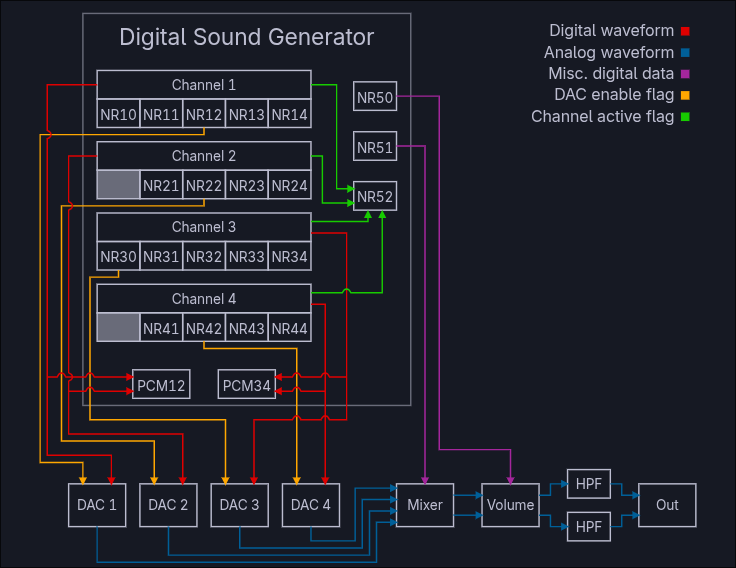
\includegraphics[width=0.65\textwidth]{imaxes/apu_details.png}
  \caption{Esquema do circuito da \acrshort{apu} \cite{pandocs}}
  \label{fig:apu-details}
\end{figure}


\subsection{Canles}
\label{subsec:apu-canles}

As catro canles comparten unha estrutura de rexistros moi semellante, con lixeiras
diferenzas segundo as capacidades de cada unha, dispoñendo todas dun rexistro de lonxitude,
que permite que a nota se deteña automaticamente tras un tempo determinado,
e dun control de frecuencia. Agás a canle 3, todas contan ademais cun envolvente de volume
que fai variar a intensidade ao longo do tempo,
necesario para efectos como as percusións ou sons con desvanecementos.

As canles 1 e 2 xeran ondas cadradas, cun ciclo de traballo seleccionable entre catro
valores, do 12,5\,\% ao 75\,\%, que altera notablemente o timbre a pesar de manter a mesma
frecuencia. A diferenza entre ambas está en que a canle 1 incorpora unha unidade de
varrido (\textit{sweep}), capaz de modificar periodicamente a súa propia frecuencia en
incrementos ou decrementos sucesivos. Este é o mecanismo detrás dos efectos de son
ascendentes e descendentes característicos da plataforma, como os saltos ou a recollida
de obxectos.

A canle 3 é a máis flexible das catro. En lugar dunha forma de onda fixa cadrada como as dúas primeiras canles,
reproduce o contido da \textit{Wave RAM},
os 16 bytes situados en \texttt{0xFF30-0xFF3F}.
Cada byte contén dous \glspl{nibble}, polo que a onda queda definida por 32 mostras de catro
bits que os xogos poden escribir libremente, o que permite aproximar calquera forma de
onda. O seu control de volume é máis limitado, xa que non dispón de envolvente e só admite
catro niveis obtidos por desprazamento das mostras.

A canle 4 xera ruído a partir dun \acrfull{lfsr}, un rexistro de desprazamento que produce
unha secuencia pseudoaleatoria de bits realimentando o seu contido mediante unha operación
lóxica. O modo de 15 bits produce un ruído de período longo, próximo ao ruído branco,
adecuado para explosións ou pasos, mentres que o de 7 bits ten un período moito máis curto
que o oído percibe como un son metálico e tonal.

\subsection{Mesturado e saída}

As saídas das catro canles combínanse nun mesturador controlado por tres rexistros.
\texttt{NR51} determina, cun bit por canle e canal, cales delas se envían á saída esquerda
e cales á dereita, o que permite un posicionamento estéreo se se empregan auriculares coa consola,
xa que a saída de audio da propia consola emprega un altofalante mono.
\texttt{NR50} axusta o volume mestre de cada canal e a mestura dun sinal de audio externo
procedente do cartucho, unha capacidade que apenas foi empregada comercialmente.
Finalmente, \texttt{NR52} permite acender e apagar por completo a \acrshort{apu} e informa,
en modo de só lectura, de cales das catro canles están activas nese momento.

A temporización de todos estes elementos non depende dun reloxo propio, senón que se deriva
do contador interno descrito na sección~\ref{sec:temporizadores}.
Un divisor coñecido como \textit{DIV-APU} xera un pulso a 512\,Hz a partir dun dos bits
dese contador, e é ese pulso o que fai avanzar os contadores de lonxitude, os envolventes
de volume e a unidade de varrido, cada un a unha fracción distinta desa frecuencia.

